\section{Implementierung}

\subsection{YOLOv5}
YOLO, ein Bilderkennungsmodell, wurde von Joseph Redmon und Ali Farhadi an der Universität von Washington entwickelt und im Jahr 2015 veröffentlicht. YOLO steht für "You Only Look Once", was darauf hinweist, dass das Modell nur einmal auf ein Bild schaut, um Objekte schnell und präzise zu erkennen. Seit seiner Veröffentlichung wurden insgesamt neun Versionen von YOLO veröffentlicht \cite{Yolo}.
\subsection{Das Modell}
Wir uns für ein vortrainiertes Modell der fünften Version von Yolo entschieden, das bereits für unsere spezifischen Anforderungen trainiert wurde. Obwohl wir mit der fünften Version eine ältere Version von YOLOv5 verwenden, bedeutet dies nicht, dass das Modell weniger effektiv ist. Für viele größen ist YOLOv5 etws schneller als zum Beispiel YOLOv8. Für uns ist die Geschwindigkeit wichtig, da wir das Model auf dem Raspberry Pi 4 laufen lassen und dort nicht viel Leistung haben.  Es kam uns daher auch zugute, das der Entwickler Yolov5s also ein kleineres Model von YOLO verwendet hat.   Der Entwickler des Modells hat Bilder aus verschiedenen Quellen gesammelt und ein eigenes benutzerdefiniertes Datenset erstellt, das aus 374 Trainingsbildern und 111 Validierungsbildern besteht.


\subsection{Makesense.ai}
Zum Labeln der Daten wurde Makesense.ai verwendet, eine Webseite für das Labeln von Bildern, die es Benutzern ermöglicht, Bilder hochzuladen und Annotationen wie Bounding Boxes und Klassifizierungen hinzuzufügen, um Datensätze für Computer Vision-Anwendungen vorzubereiten \cite{noauthor_make_nodate}. Der Entwickler hat die Daten in drei Klassen unterteilt: 'walking', 'sitting' und 'fall detected' (sieh Abbildung \ref{fig:yolo_classes}).

\begin{figure}[H]
	\centering
	\begin{minipage}[b]{0.3\textwidth}
		\centering
		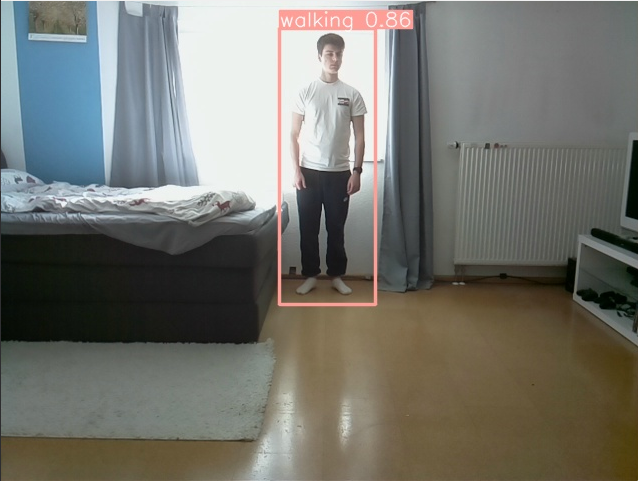
\includegraphics[width=\textwidth]{images/walking.png}
		\caption*{Klasse: ''walking''}
	\end{minipage}
	\hfill
	\begin{minipage}[b]{0.3\textwidth}
		\centering
		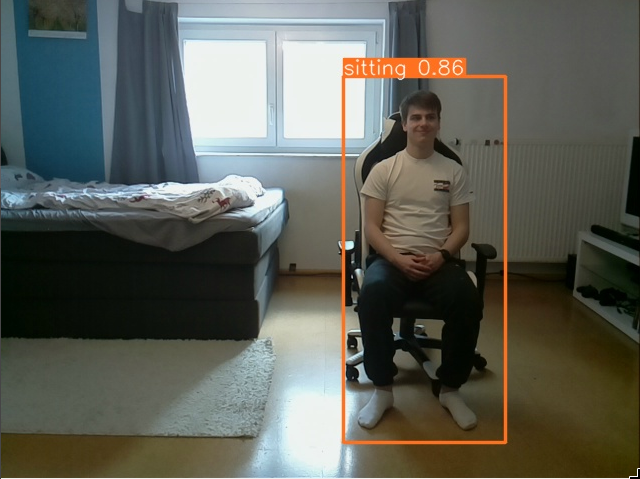
\includegraphics[width=\textwidth]{images/sitting.png}
		\caption*{Klasse: ''sitting''}
	\end{minipage}
	\hfill
	\begin{minipage}[b]{0.3\textwidth}
		\centering
		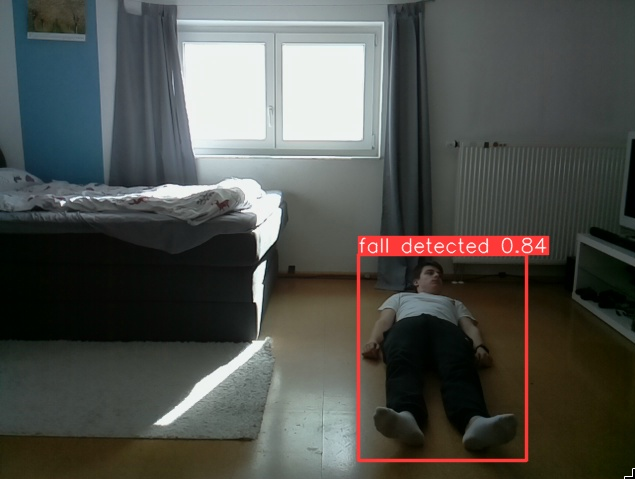
\includegraphics[width=\textwidth]{images/fallen.png}
		\caption*{Klasse: ''fall detected''}
	\end{minipage}
	\caption{YOLOv5 Detektion Klassen}
	\label{fig:yolo_classes}
\end{figure}



\subsection{Anbindung}
Die Anbindung an das YOLOv5-Modell erfolgt über PyTorch, ein Open-Source-Framework für maschinelles Lernen, das auf der Programmiersprache Python und der Torch-Bibliothek basiert. PyTorch wurde 2016 von einem Forscherteam für künstliche Intelligenz bei Facebook entwickelt \cite{noauthor_pytorch_nodate}.

Das Modell läuft in einem Docker-Container, der kontinuierlich über MQTT einen boolean-Wert veröffentlicht, um anzuzeigen, ob ein Alarm aufgetreten ist. Zur Einbindung der Raspberry Pi Kamera verwendet der Container auch OpenCV, eine Open-Source-Bibliothek für Computer Vision \cite{OpenCV}. Mithilfe von OpenCV wurde auch eine Funktion entwickelt, die über MQTT ein Bild mit allen Detektionen versendet. Diese Bilder können später mithilfe eines weiteren Docker Containers   einem lokalen Rechner angezeigt werden.


\subsection{Evaluation}
Das Modell soll dem Model-Entwickler zufolge eine Genauigkeit von 85 bis 90\% bei Tageslicht haben. Es hat jedoch Schwierigkeiten mit der Detektion von vielen Personen auf einem Bild, was zu falschen Erkennungen führen kann. Für unseren Anwendungsfall, die Überwachung von Patienten, ist dies jedoch kein Problem, da wir in unseren Bildern normalerweise nur einzelne Patienten haben. 


\section{Matrix}

Matrix ist ein offener Standard für interoperable, dezentrale, Echtzeitkommunikation über das Internetprotokoll (IP). Benutzer verbinden sich mit einem eigenen Server (Heimserver) und können Räume auf jedem Matrix-Server betreten, was die Kommunikation über Server hinweg ermöglicht. Nachrichten werden zwischen den Servern synchronisiert, was eine unterbrechungsfreie Kommunikation ermöglicht, selbst wenn ein Server offline geht. Matrix bietet Ende-zu-Ende-Verschlüsselung für sichere Gespräche. Um Matrix auszuprobieren, kann man einen der zahlreichen  Matrix-Clients verwenden \cite{noauthor_introduction_nodate}.  Wir haben auch für Matrix ein Docker Container verwendet, um den einen homserver auszusetzen \cite{noauthor_matrixdotorgsynapse_nodate}.  Wir nutzen Matrix, um die Pfleger über einen Alarm zu informieren. 

\subsection{Element}
Für unsere Kommunikation haben wir uns für den Matrix-Client Element entschieden \cite{noauthor_element_nodate}. Element wird von den Entwicklern von Matrix geleitet und bietet eine benutzerfreundliche Oberfläche sowie eine Vielzahl von Funktionen, die für unsere Bedürfnisse ideal sind. 


\subsection{Nginx reverse proxy}

Damit unser Matrix-Server auch eine SSL verwneden kann benötigen wir einen Reverse-Proxy. Ein Reverse-Proxy fungiert als Vermittler zwischen Clients (z.B. Webbrowsern) und Webservern. Anstatt direkt mit dem Ursprungsserver zu kommunizieren, senden Clients ihre Anfragen an den Reverse-Proxy, der diese dann an den richtigen Server weiterleitet und die Antworten zurück an die Clients sendet \cite{noauthor_was_nodate}. Man kann dies aus Aspekten der Sicherheit, der Performance oder der Zuverlässigkeit tun. Wir haben für unsere Implementierung den Nginx als reverse proxy verwendet \cite{noauthor_nginx_nodate}, da der  Server gut und weit verbreitetet dokumentiert ist. Der Nginx ist als Docker-Container verfügbar, was uns die Integration  erleichtert hat \cite{noauthor_nginx_nodate}. 


\begin{figure}[H]
\begin{tikzpicture}[scale=0.8]
	
		\node[inner sep=0pt] (whitehead) at (-10,2)
	{
\includegraphics[width=0.15\textwidth]{images/computer.png}};
	
	\node[font=\scriptsize] at (-10,1.2) {\scriptsize Laptop 1} ;
	
	\draw[->] (-9.2,1.8)--(-6.5,0.5) node[pos=0.5, above,rotate=-28] { \scriptsize example.org};
	
		\node[inner sep=0pt] (whitehead) at (-10,0)
	{
\includegraphics[width=0.15\textwidth]{images/computer.png}};
	
		\node[font=\scriptsize] at (-10,-0.8) {\scriptsize Laptop 2};
	
		\draw[->] (-9,0)--(-6.5,0) node[pos=0.45, above] { \scriptsize example.org};
	
		\node[inner sep=0pt] (whitehead) at (-10,-2)
	{
\includegraphics[width=0.15\textwidth]{images/computer.png}};
	
			\node[font=\scriptsize] at (-10,-2.8) {\scriptsize Laptop 3};
	
		\draw[->] (-9.2,-1.8)--(-6.5,-0.5)  node[pos=0.5, above,rotate=28] { \scriptsize example.org};
	
		\node[inner sep=0pt] (whitehead) at (-5,0)
	{
\includegraphics[width=0.10\textwidth]{images/cloud.png}};
	
				\node[font=\scriptsize] at (-5,-0.8) {\scriptsize Internet};
	
		\draw[->] (-4,0)--(-1,-0);
	
	\node[inner sep=0pt] (whitehead) at (0,0)
	{
\includegraphics[width=0.10\textwidth]{images/switch.png}};
	
		\node[font=\scriptsize] at (0,-0.8) {\scriptsize reverse proxy};
	
	\draw[->] (1,0.2)--(4,0.8);
	
		\draw[->] (1,-0.2)--(4,-0.8);
	
		\node[inner sep=0pt] (whitehead) at (5,1)
	{
\includegraphics[width=0.10\textwidth]{images/switch.png}};
	
			\node[font=\scriptsize] at (5,0.4) {\scriptsize matrix server};
	
			\node[inner sep=0pt] (whitehead) at (5,-1)
	{
\includegraphics[width=0.10\textwidth]{images/switch.png}};
	
		\node[font=\scriptsize] at (5,-1.6) {\scriptsize mail server};
	
\end{tikzpicture}
	\caption{Aufbau eiens reverse proxies}
\label{fig:patient_reverse_proxy}
\end{figure}

\subsection{Postgres}
Es wird empfohlen, den Matrix Docker-Container mit PostgreSQL einzurichten (siehe \cite{noauthor_installation_nodate}). Standardmäßig wird SQLite als Datenbank verwendet, da dies die Einrichtung erleichtert. Aus Gründen der Leistungsoptimierung wird jedoch empfohlen, PostgreSQL zu verwenden, da es besser optimiert ist.  PostgreSQL ist ein leistungsstarkes,  Datenbanksystem, das SQL verwendet und erweitert. Es bietet viele Funktionen zur sicheren Speicherung und Skalierung komplexer Datenlasten. Entwickelt wurde es im Rahmen des POSTGRES-Projekts an der University of California in Berkeley.\cite{noauthor_postgresql_nodate}

\subsection{Certbot}
Um sicherzustellen, dass unser Matrixserver SSL-Verschlüsselung unterstützt, benötigen wir ein SSL-Zertifikat.  SSL (Secure Sockets Layer) ist eine Technologie zur Sicherung von Internetverbindungen durch Verschlüsselung der Daten zwischen Browsern und Servern, um die Vertraulichkeit und Integrität sensibler Informationen wie persönlicher und finanzieller Daten zu gewährleisten. Es ermöglicht auch die Authentifizierung des Servers gegenüber dem Browser, um sicherzustellen, dass die Verbindung mit der richtigen Website hergestellt wird und nicht von Angreifern manipuliert wird \cite{SSL}. Certbot ist ein benutzerfreundlicher Client, der ein Zertifikat von Let's Encrypt abruft.  Das SSL-Zertifikat von Let's Encrypt ist kostenlos. 

\subsection{Matrix Bridge}
Um unseren E-Mail-Server mit Matrix zu verbinden, haben wir eine Matrix-Bridge genutzt \cite{jojii_jojiiofficialmatrix-emailbridge_2024}. Bridges in Matrix ermöglichen die Verbindung mit anderen Plattformen und fördern somit die Interoperabilität. Durch sie kann Matrix über verschiedene digitale Landschaften hinweg vernetzt werden \cite{noauthor_bridges_nodate}. Unsere Bridge ermöglicht es uns, E-Mails über Matrix zu senden und über E-Mail in Matrix erreichbar zu sein. Wir verwenden die Bridge, um Alarme nur über E-Mail auszulösen, die dann automatisch auch in Matrix gesendet werden.
